\chapter{IMPLEMENTAÇÃO DAS TÉCNICAS E ANÁLISE DOS RESULTADOS}\label{ch:implementacao}

\section{INTRODUÇÃO}
Este capítulo tem como finalidade apresentar com um maior nível de detalhamento as técnicas utilizadas neste trabalho, com o objetivo de se atingir as metas propostas já descritas no Capítulo~\ref{ch:introducao}, no item~\ref{sec:objetivos}.

\section{COLETA DE DADOS}
Uma característica comentada anteriormente sobre a rede social \textit{Twitter} é a disponibilidade de informações de eventos em tempo real. Os \textit{tweets} podem ser postados com o intuito de comentar sobre a final de um campeonato de futebol, datas importantes, acontecimentos internacionais e políticos, entre outros.

Para este trabalho foi aproveitado o dia 17 de abril de 2016, onde foi realizado a votação do Congresso Brasileiro pela continuação do processo de Impeachment do cargo da presidenta Dilma Rouseff. Neste dia milhares de \textit{tweets} foram publicados utilizando a \textit{hashtag} "\#ImpeachmentDay" \space com o objetivo de comentar sobre o evento de votação e, também, a atual situação política do Brasil.

Com o objetivo de coletar todos os dados que contenham a \textit{hashtag} "\#ImpeachmentDay", foi desenvolvido um \textit{script} que utiliza o serviço de \textit{Stream} do \textit{Twitter} também conhecido como \textit{FireHose}.

As primeiras linhas do \textit{script} servem para importar as bibliotecas e objetos necessários para a utilização da API do \textit{Twitter}, assim como as informações das chaves de acesso e \textit{tokens} para o protocolo OAuth, que são fundamentais para a comunicação com o serviço de \textit{Stream}. \\


\lstset{language=Python}
\begin{lstlisting}
from tweepy.streaming import StreamListener
from tweepy import OAuthHandler
from tweepy import Stream

access_token = "131556934-LrYRiXzAL3QcRyFN0fdN53EDWhNGfZFnVX59NCnT"
access_token_secret = "JraMtps5lB98d8XoelAF71KHn8ZQ4nshdoSKiFlTz6OHd"
consumer_key = "P4XZ2GUkeqdhIlQMOredBuW05"
consumer_secret = "r5TPb2UcM8bzxq7t5zflRPMHUrCfwNG4GRuVPXypowrpHhTmue"


class StdOutListener(StreamListener):

    def on_data(self, data):
        print data
        return True

    def on_error(self, status):
        print status


if __name__ == '__main__':

    l = StdOutListener()
    auth = OAuthHandler(consumer_key, consumer_secret)
    auth.set_access_token(access_token, access_token_secret)
    stream = Stream(auth, l)

    stream.filter(track=['ImpeachmentDay'])
\end{lstlisting}

Na linha 11 é criado uma classe que irá instanciar um serviço de escuta para este \textit{Stream}. O serviço de escuta é responsável por observar todos os \textit{tweets} que são publicados e após identificar no \textit{tweet} alguma palavra ou a \textit{hashtag} semelhante a palavra declarada na linha 28, é então capturado este \textit{tweet} e impresso na tela de execução do \textit{script}.

Quando este \textit{script} está em execução é mostrado na tela todos os \textit{tweets} que estão sendo coletados, já filtrados, porém não está sendo persistido em nenhum arquivo ou banco de dados. Com o intuito de salvar todos estes dados foi utilizado o comando "$>$", conhecido como \textit{stdout}, presente em sistemas operacionais de base \textit{Unix}. O comando "$>$" \space permite redirecionar a saída do código anterior, no caso a execução do \textit{script} "coletar-hashtags.py", para um novo arquivo ou um arquivo já existente conforme ilustrado pela Figura~\ref{exec-coleta}.

\begin{figure}[h]
	\centering
	\fbox{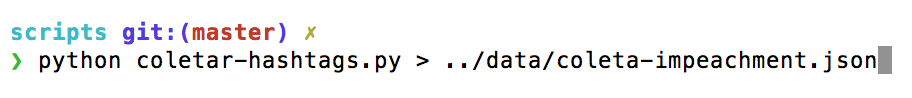
\includegraphics[width=0.95\textwidth]{Cap5/imagens/execucao-script}}
	\caption{Execução do \textit{script} para coleta de dados}
	\vspace{-0.3cm}
	\legend{FONTE: Elaborado pelo autor}
	\label{exec-coleta}
\end{figure}

O \textit{script} de coleta de dados permaneceu em execução durante 14 horas (das 08:30 às 22:30) do dia 17 de abril, concluindo em um arquivo de 2.6 gigabytes. O formato deste arquivo é um JSON onde apresenta todas as informações presentes em um \textit{tweet}, demonstrado através do seguinte código: \\ \\

\begin{lstlisting}
{
    "created_at": "Sun Apr 17 15:15:21 +0000 2016",
    "id": 721718699418202112,
    "id_str": "721718699418202112",
    "text": "RT @GarotaCiume: N\u00e3o sou petista, s\u00f3 n\u00e3o sou cega. Impeachment sem crime de responsabilidade \u00e9 golpe, e voc\u00eas est\u00e3o traindo a democracia. #\u2026",
    "source": "\u003ca href=\"http:\/\/twitter.com\/download\/android\" rel=\"nofollow\"\u003eTwitter for Android\u003c\/a\u003e",
    "truncated": false,
    "in_reply_to_status_id": null,
    "in_reply_to_status_id_str": null,
    "in_reply_to_user_id": null,
    "in_reply_to_user_id_str": null,
    "in_reply_to_screen_name": null,
    "user": {
        "id": 1876843824,
        "id_str": "1876843824",
        "name": "Millena Souza",
        "screen_name": "Souzaa_mih1",
        "location": "Brasil, Vit\u00f3ria- ES",
        "url": "https:\/\/www.facebook.com\/myllena.souzaa",
        "description": "Brasileira 15 , paulista e capixaba, feminista,Taurina e n\u00e3o sou obrigada a nada  \u2764\u2764 BORN TO DIE !!",
        "protected": false,
        "verified": false,
        "followers_count": 433,
        "friends_count": 431,
        "listed_count": 0,
        "favourites_count": 613,
        "statuses_count": 28370,
        "created_at": "Tue Sep 17 20:52:04 +0000 2013",
        "utc_offset": -10800,
        "time_zone": "Brasilia",
        "geo_enabled": true,
        "lang": "pt",
        "contributors_enabled": false,
        "is_translator": false,
        "profile_background_color": "611994",
        "profile_background_image_url": "http:\/\/pbs.twimg.com\/profile_background_images\/378800000076733988\/60df12d5296d8d8081e19c306c15c859.jpeg",
        "profile_background_image_url_https": "https:\/\/pbs.twimg.com\/profile_background_images\/378800000076733988\/60df12d5296d8d8081e19c306c15c859.jpeg",
        "profile_background_tile": true,
        "profile_link_color": "6B25C7",
        "profile_sidebar_border_color": "FFFFFF",
        "profile_sidebar_fill_color": "7AC3EE",
        "profile_text_color": "3D1957",
        "profile_use_background_image": true,
        "profile_image_url": "http:\/\/pbs.twimg.com\/profile_images\/699081483546443776\/uCBDXAfO_normal.jpg",
        "profile_image_url_https": "https:\/\/pbs.twimg.com\/profile_images\/699081483546443776\/uCBDXAfO_normal.jpg",
        "profile_banner_url": "https:\/\/pbs.twimg.com\/profile_banners\/1876843824\/1455509034",
        "default_profile": false,
        "default_profile_image": false,
        "following": null,
        "follow_request_sent": null,
        "notifications": null
    },
    "geo": null,
    "coordinates": null,
    "place": null,
    "contributors": null,
    "retweeted_status": {
        "created_at": "Sun Apr 17 15:07:13 +0000 2016",
        "id": 721716654569349121,
        "id_str": "721716654569349121",
        "text": "N\u00e3o sou petista, s\u00f3 n\u00e3o sou cega. Impeachment sem crime de responsabilidade \u00e9 golpe, e voc\u00eas est\u00e3o traindo a democracia. #ImpeachmentDay",
        "source": "\u003ca href=\"http:\/\/twitter.com\/download\/iphone\" rel=\"nofollow\"\u003eTwitter for iPhone\u003c\/a\u003e",
        "truncated": false,
        "in_reply_to_status_id": null,
        "in_reply_to_status_id_str": null,
        "in_reply_to_user_id": null,
        "in_reply_to_user_id_str": null,
        "in_reply_to_screen_name": null,
        "user": {
            "id": 206181302,
            "id_str": "206181302",
            "name": "Garota Ci\u00fame",
            "screen_name": "GarotaCiume",
            "location": "snapchat \/\/ leuncosta \u2728",
            "url": "http:\/\/Instagram.com\/leuncosta",
            "description": "Ciume \u00e9 igual bater o dedinho do p\u00e9 no sof\u00e1: coisa boba, mas d\u00f3i demais. \u2022 contato: contatogarotaciume@gmail.com",
            "protected": false,
            "verified": false,
            "followers_count": 1202807,
            "friends_count": 139,
            "listed_count": 383,
            "favourites_count": 40277,
            "statuses_count": 25882,
            "created_at": "Fri Oct 22 12:52:10 +0000 2010",
            "utc_offset": -10800,
            "time_zone": "Brasilia",
            "geo_enabled": true,
            "lang": "pt",
            "contributors_enabled": false,
            "is_translator": false,
            "profile_background_color": "FFFFFF",
            "profile_background_image_url": "http:\/\/pbs.twimg.com\/profile_background_images\/879103282\/2454b176f3fffc4b100fb2bc64b1f2b5.png",
            "profile_background_image_url_https": "https:\/\/pbs.twimg.com\/profile_background_images\/879103282\/2454b176f3fffc4b100fb2bc64b1f2b5.png",
            "profile_background_tile": false,
            "profile_link_color": "383838",
            "profile_sidebar_border_color": "FFFFFF",
            "profile_sidebar_fill_color": "F6F6F6",
            "profile_text_color": "000000",
            "profile_use_background_image": true,
            "profile_image_url": "http:\/\/pbs.twimg.com\/profile_images\/3719404815\/b868778f39b4b087561e3444b3093e20_normal.gif",
            "profile_image_url_https": "https:\/\/pbs.twimg.com\/profile_images\/3719404815\/b868778f39b4b087561e3444b3093e20_normal.gif",
            "profile_banner_url": "https:\/\/pbs.twimg.com\/profile_banners\/206181302\/1403658723",
            "default_profile": false,
            "default_profile_image": false,
            "following": null,
            "follow_request_sent": null,
            "notifications": null
        },
        "geo": null,
        "coordinates": null,
        "place": null,
        "contributors": null,
        "is_quote_status": false,
        "retweet_count": 153,
        "favorite_count": 130,
        "entities": {
            "hashtags": [{
                "text": "ImpeachmentDay",
                "indices": [121, 136]
            }],
            "urls": [],
            "user_mentions": [],
            "symbols": []
        },
        "favorited": false,
        "retweeted": false,
        "filter_level": "low",
        "lang": "pt"
    },
    "is_quote_status": false,
    "retweet_count": 0,
    "favorite_count": 0,
    "entities": {
        "hashtags": [{
            "text": "ImpeachmentDay",
            "indices": [139, 140]
        }],
        "urls": [],
        "user_mentions": [{
            "screen_name": "GarotaCiume",
            "name": "Garota Ci\u00fame",
            "id": 206181302,
            "id_str": "206181302",
            "indices": [3, 15]
        }],
        "symbols": []
    },
    "favorited": false,
    "retweeted": false,
    "filter_level": "low",
    "lang": "pt",
    "timestamp_ms": "1460906121483"
}
\end{lstlisting}


\section{ANÁLISE DE DADOS}
Após a coleta de dados foi gerado, então, um arquivo JSON de 2.6 gigabytes. Portanto a próxima etapa será analisar estes dados para extrair informações úteis.

Foi realizado testes no arquivo JSON coletado para verificar se existe algum tipo de \textit{dirty data}, que são informações quebradas, dados irrelevantes ou códigos que impedem a execução de \textit{scripts} de mineração \cite{dirty-data}. A Figura~\ref{fig-dirty} demonstra o único padrão de \textit{dirty data} encontrado dentro do arquivo.

\begin{figure}[h]
	\centering
	\fbox{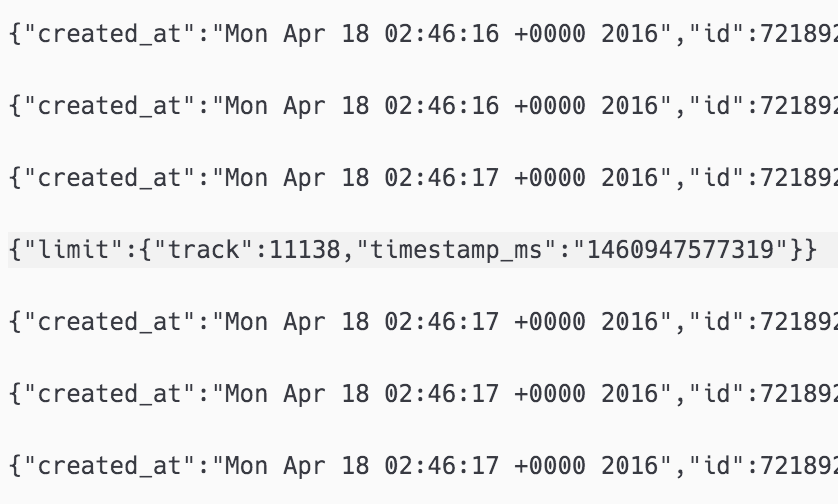
\includegraphics[width=0.95\textwidth]{Cap5/imagens/limit}}
	\caption{\textit{Dirty Data} presente no arquivo coletado}
	\vspace{-0.3cm}
	\legend{FONTE: Elaborado pelo autor}
	\label{fig-dirty}
\end{figure}

Dentro das milhares linhas do arquivo existem algumas linhas contendo este mesmo padrão de \textbf{\{"limit":} que foram removidos utilizando outra ferramenta de sistemas baseados em Unix, o \textit{grep}.

A ferramenta \textit{grep} é um canivete suíço para o uso de expressões regulares e possui uma funcionalidade que permite realizar uma consulta inversa, ou seja, o usuário passa um padrão ou uma palavra que se deseja encontrar dentro de um determinado arquivo, e após encontrar todas as ocorrências o \textit{grep} seleciona tudo o que não contém este padrão ou palavra.

Combinado com o comando de \textit{stdout} ($>$), é possível redirecionar todos os dados que não possui este tipo de \textit{dirty data} para um novo arquivo conforme a Figura~\ref{limpa-dado}.

\begin{figure}[h]
	\centering
	\fbox{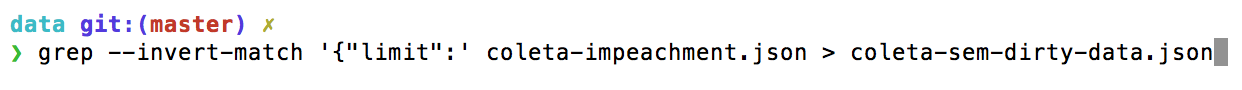
\includegraphics[width=0.95\textwidth]{Cap5/imagens/grep}}
	\caption{Utilizando o comando \textit{grep} para gerar um novo arquivo sem \textit{dirty data}}
	\vspace{-0.3cm}
	\legend{FONTE: Elaborado pelo autor}
	\label{limpa-dado}
\end{figure}

Tendo então um arquivo JSON sem a presença de \textit{dirty data} é possível iniciar o processo de extração de conhecimento utilizando o interpretador \textit{IPython}.

Nesta primeira etapa importa-se as bibliotecas necessárias para se trabalhar com arquivos do tipo JSON e também para a geração de gráficos, conforme o código a seguir: \\

\begin{lstlisting}
%matplotlib inline

import json
import pandas as pd
import matplotlib.pyplot as plt


tweets_data_path = 'data/coleta-sem-dirty-data.json'

tweets_data = []
tweets_file = open(tweets_data_path, "r")
for line in tweets_file:
    try:
        tweet = json.loads(line)
        tweets_data.append(tweet)
    except:
        continue

tweets = pd.DataFrame()
print len(tweets_data)
\end{lstlisting}

A primeira linha deste código permite a visualização de gráficos e planilhas no \textit{IPython}. Na linha 8 em diante está sendo realizado a construção de um \textit{DataFrame}, que é definido no Capítulo~\ref{ch:materiais-metodos}, seção~\ref{pandas}, através leitura do arquivo "coleta-sem-dirty-data.json".

A execução deste código permite, então, gerar um \textit{DataFrame} e informar o número de \textit{tweets} que ele contém. Esses \textit{DataFrames} possuem uma arquitetura semelhante ao formato de tabelas (linhas e colunas) em que é possível adicionar uma coluna ou uma tabela a uma variável em Python. Através do mapeamento de uma condição em um \textit{DataFrame}, apresentado no código seguinte para mapear o texto, a língua e o país em que o \textit{tweet} foi publicado. \\

\begin{lstlisting}
tweets['text'] = map(lambda tweet: tweet['text'], tweets_data)
tweets['lang'] = map(lambda tweet: tweet['lang'], tweets_data)
tweets['country'] = map(lambda tweet: tweet['place']['country']
						if tweet['place'] != None else None, tweets_data)

tweets_by_lang = tweets['lang'].value_counts()

fig, ax = plt.subplots(figsize=(20,10))
ax.tick_params(axis='x', labelsize=20)
ax.tick_params(axis='y', labelsize=15)
ax.set_xlabel('Linguas'.decode('utf-8'), fontsize=20)
ax.set_ylabel('Numero de tweets'.decode('utf-8') , fontsize=20)
ax.set_title('Top 4 Linguas'.decode('utf-8'),
				fontsize=20, fontweight='bold')
tweets_by_lang[:4].plot(ax=ax, kind='bar', color='mediumspringgreen')
plt.grid()
\end{lstlisting}

Após o mapeamento das informações do \textit{DataFrame} foi feito um gráfico para medir a quantidade de \textit{tweets} em relação as 04 línguas mais \textit{tweetadas}. A Figura~\ref{lingua} apresenta o gráfico gerado.

\begin{figure}[h]
	\centering
	\fbox{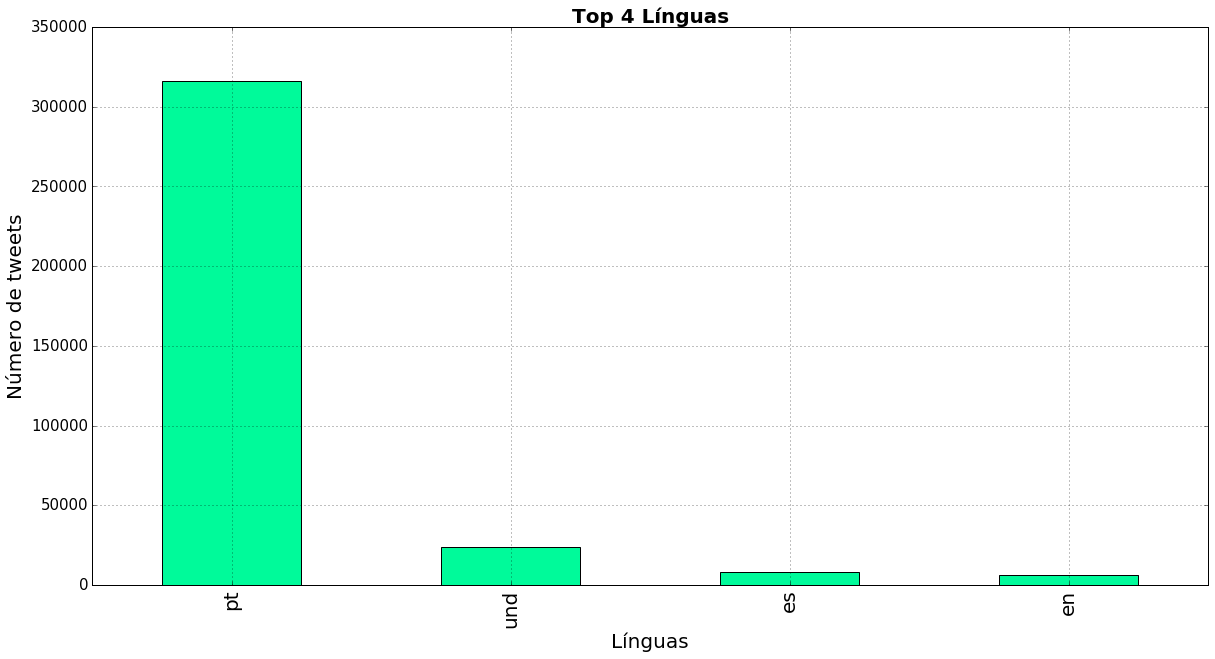
\includegraphics[width=1\textwidth]{Cap5/graficos/linguas}}
	\caption{Línguas que mais realizaram \textit{tweets}}
	\vspace{-0.3cm}
	\legend{FONTE: Elaborado pelo autor}
	\label{lingua}
\end{figure}

É possível verificar que existe uma barra com o nome de \textit{und} para especificar a segunda língua que realizou mais \textit{tweets}. Essa é uma condição em que não foi identificada a língua de origem e então a API do \textit{Twitter} classifica como \textit{undefined}, ou indefinido no português. Essa linguagem indefinida ocorre devido ao \textit{software} em que o usuário está realizando o \textit{tweet}, por exemplo um navegador \textit{web}, um aplicativo \textit{mobile} do \textit{Twitter} ou algum aplicativo de terceiro que permite realizar ações no \textit{Twitter}. Caso a linguagem não está definida nestes ambientes a API o classifica como \textit{undefined}.

Semelhante ao código anterior é possível verificar quais os países que estão comentando sobre a \textit{hashtag} "\#ImpeachmentDay". \\ \\

\begin{lstlisting}
tweets_by_country = tweets['country'].value_counts()

fig, ax = plt.subplots(figsize=(20,10))
ax.tick_params(axis='x', labelsize=15)
ax.tick_params(axis='y', labelsize=15)
ax.set_xlabel('Paises'.decode('utf-8'), fontsize=20)
ax.set_ylabel('Numero de tweets'.decode('utf-8') , fontsize=20)
ax.set_title('Top 5 Paises'.decode('utf-8'), fontsize=20, fontweight='bold')
tweets_by_country[:5].plot(ax=ax, kind='bar', color='lightskyblue')
plt.grid()
\end{lstlisting}

O código acima verifica quais são os 05 países que mais realizaram \textit{tweets} através do mapeamento do \textit{DataFrame} e então gera o gráfico representado na Figura~\ref{paises}.

\begin{figure}[h]
	\centering
	\fbox{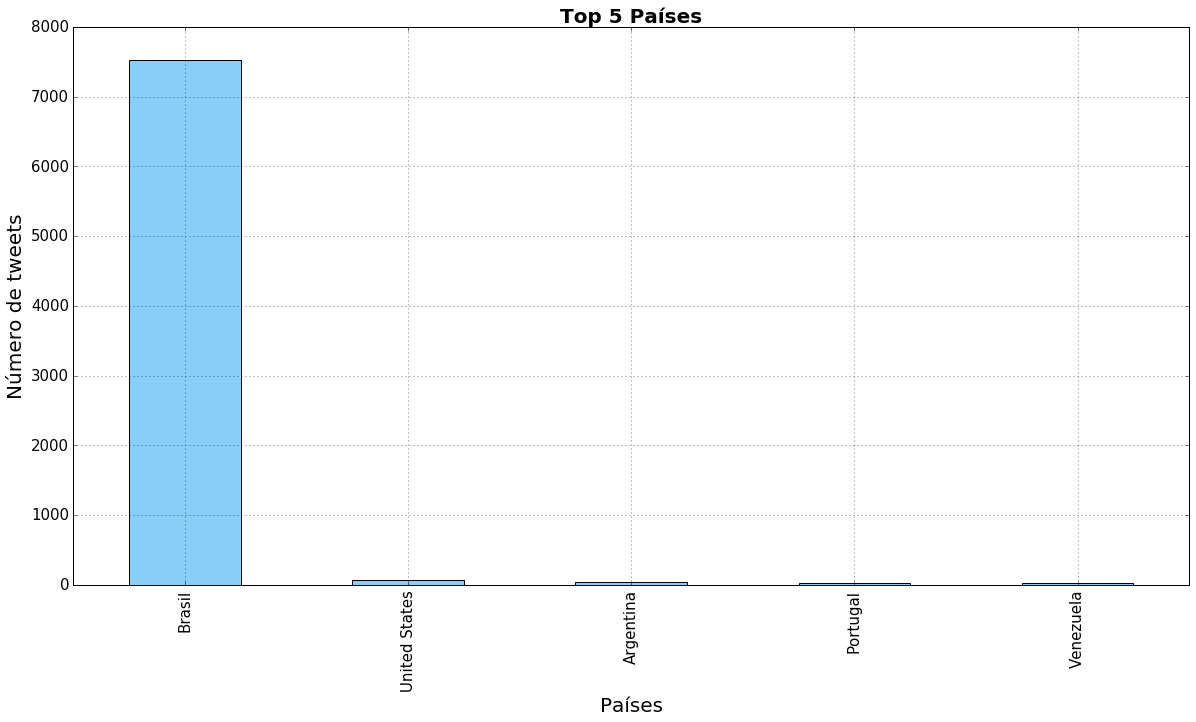
\includegraphics[width=1\textwidth]{Cap5/graficos/paises}}
	\caption{Países que mais realizaram \textit{tweets}}
	\vspace{-0.3cm}
	\legend{FONTE: Elaborado pelo autor}
	\label{paises}
\end{figure}

Este gráfico demonstra claramente que a maior parte dos \textit{tweets} foram publicados do Brasil e apenas uma pequena quantia deles foram realizados nos Estados Unidos, Argentina, Portugal e Venezuela. É importante notar que nem todos os \textit{tweets} gerados possuem um país de origem semelhante a situação anterior onde a API do \textit{Twitter} os classificam como \textit{undefined}, porém não é apresentado neste gráfico.

\begin{lstlisting}
import re


def word_in_text(word, text):
    word = word.lower()
    text = text.lower()
    match = re.search(word, text)
    if match:
        return True
    return False

tweets['NaoVaiTerGolpe'] = tweets['text'].apply(lambda tweet: word_in_text('NaoVaiTerGolpe', tweet))
tweets['TchauQuerida'] = tweets['text'].apply(lambda tweet: word_in_text('TchauQuerida', tweet))
tweets['ForaDilma'] = tweets['text'].apply(lambda tweet: word_in_text('ForaDilma', tweet))
tweets['BrasilContraOGolpe'] = tweets['text'].apply(lambda tweet: word_in_text('BrasilContraOGolpe', tweet))
tweets['ForaCunha'] = tweets['text'].apply(lambda tweet: word_in_text('ForaCunha', tweet))

# print tweets['FicaQuerida'].value_counts()[True]
# print tweets['NaoVaiTerGolpe'].value_counts()[True]
# print tweets['ForaPT'].value_counts()[True]

hashtags = ['ForaDilma', 'NaoVaiTerGolpe', 'TchauQuerida', 'BrasilContraOGolpe', 'ForaCunha']
tweets_by_hashtags = [tweets['ForaDilma'].value_counts()[True],
                      tweets['NaoVaiTerGolpe'].value_counts()[True],
                      tweets['TchauQuerida'].value_counts()[True],
                      tweets['BrasilContraOGolpe'].value_counts()[True],
                      tweets['ForaCunha'].value_counts()[True]]

plt.subplots(figsize=(9,9))
colors = ['gold', 'yellowgreen', 'lightcoral', 'lightskyblue', 'peachpuff']
explode = (0.03, 0.03, 0.03, 0.05, 0.03)
plt.pie(tweets_by_hashtags, explode=explode, labels=hashtags, colors=colors,
        autopct='%1.1f%%', shadow=True, startangle=140)
plt.rcParams['font.size'] = 12
plt.legend(tweets_by_hashtags, loc=(1,.6))
plt.axis('equal')
plt.show()
\end{lstlisting}

































